\section{Results}
\label{sec:results}

We found that our algorithm created trajectories that were free of collisions and produced smooth motion. Below we have a diagram showing the patch in various steps of our algorithm. Next we show the final curved trajectories with various sized input. Lastly we show some performance tests.

\devin{the images are not lining up how I want them too.}

\begin{figure}[H]
 \centering
 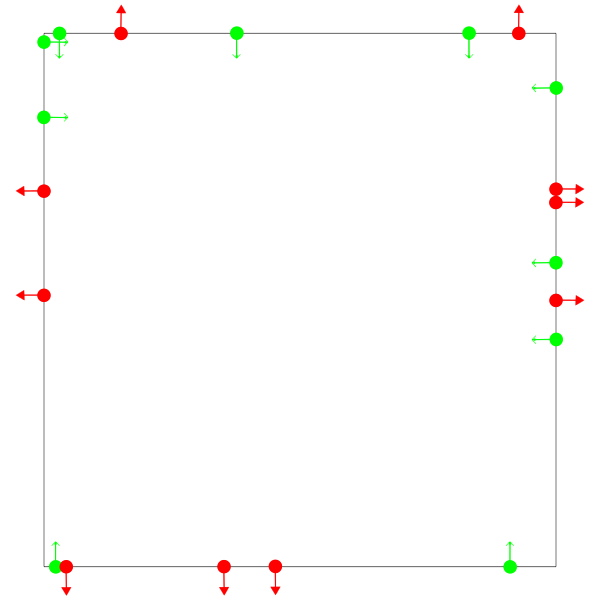
\includegraphics[width=3in]{images/steps-input.png}
 \caption{caption caption caption}
\end{figure}

\begin{figure}[H]
 \centering
 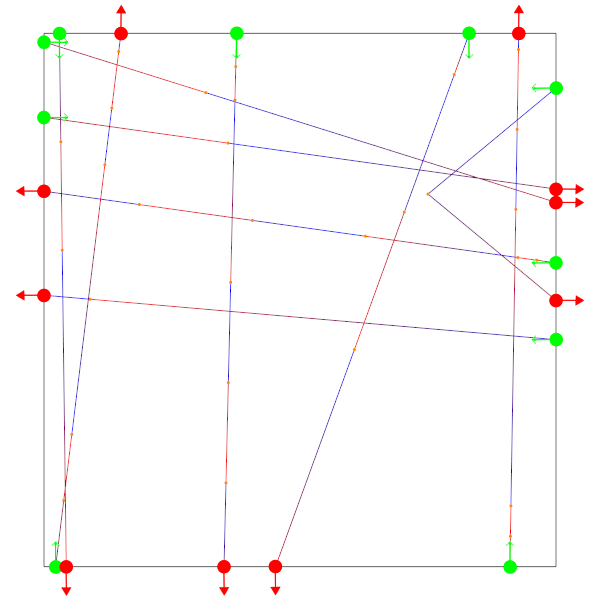
\includegraphics[width=3in]{images/steps-connected.png}
 \caption{caption caption caption}
\end{figure}

\begin{figure}[H]
 \centering
 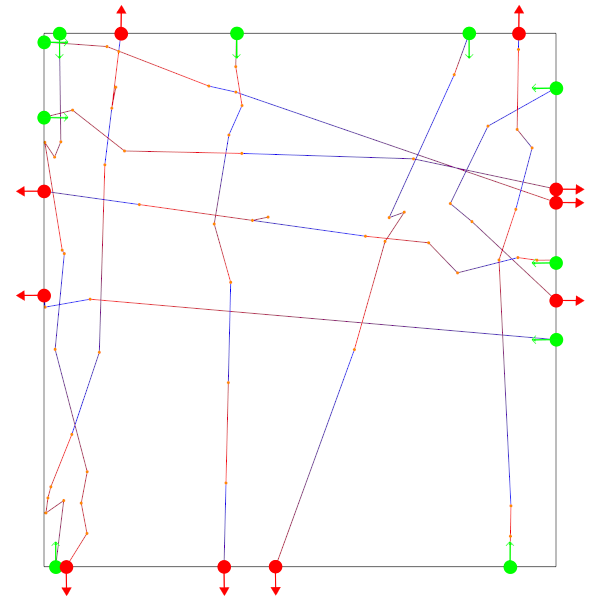
\includegraphics[width=3in]{images/steps-collisionFree.png}
 \caption{caption caption caption}
\end{figure}

\begin{figure}[H]
 \centering
 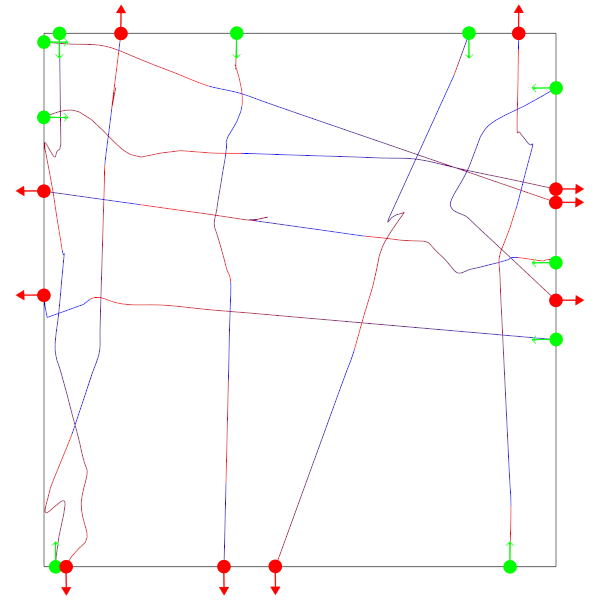
\includegraphics[width=3in]{images/steps-smoothed.png}
 \caption{caption caption caption}
\end{figure}


The performance was measured on a computer with a quad core 2.8 GHz processor and 8GB of RAM. We found trajectories for patches with randomly generated entry and exit points. The patches all had base square of size 16 by 16. The period was 10 seconds. There were 20 samples for each number of agents between 1 and 50 for a total of 1000 samples. 994 of these were collision free. The other 6 were stopped after they reached 2000 iterations. We recorded the number of iterations required for collision free trajectories as well as the computation time in seconds.

\begin{figure}[H]
 \centering
 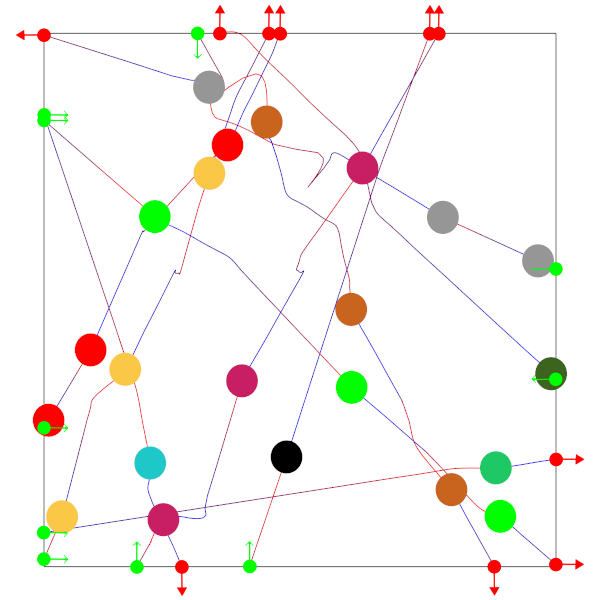
\includegraphics[width=3in]{images/res-10-entry-exit.png}
 \caption{caption caption caption}
\end{figure}

\begin{figure}[H]
 \centering
 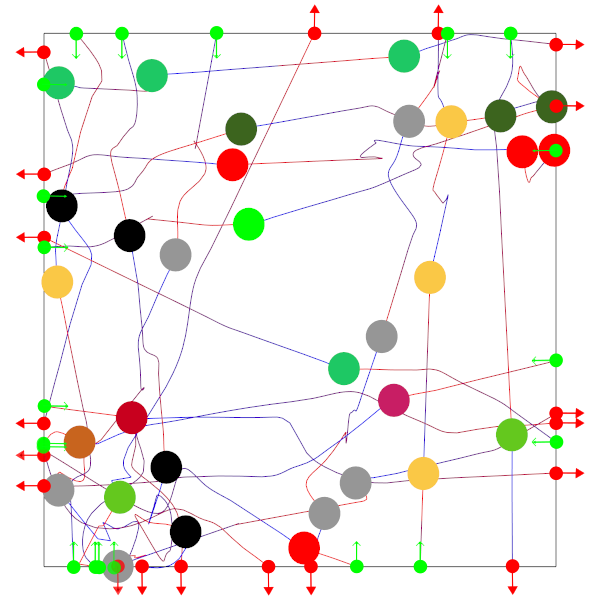
\includegraphics[width=3in]{images/res-20-entry-exit.png}
 \caption{caption caption caption}
\end{figure}

\begin{figure}[H]
 \centering
 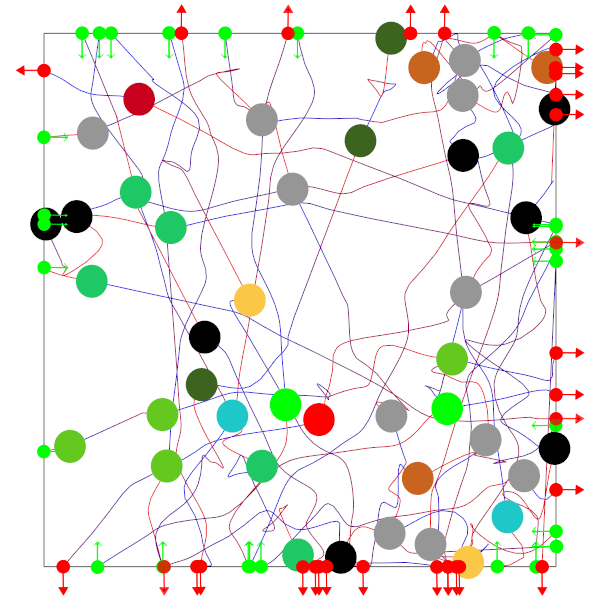
\includegraphics[width=3in]{images/res-30-entry-exit.png}
 \caption{caption caption caption}
\end{figure}

\begin{figure}[H]
 \centering
 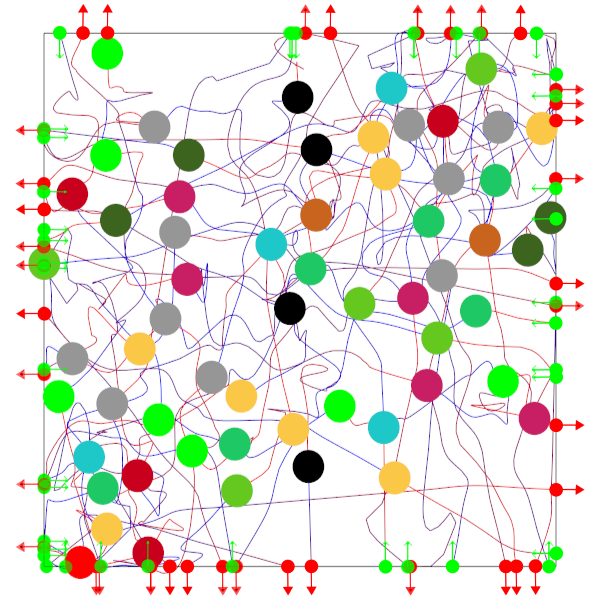
\includegraphics[width=3in]{images/res-40-entry-exit.png}
 \caption{caption caption caption}
\end{figure}



\begin{figure}[H]
 \centering
 \includegraphics[width=3in]{images/res-iter-graph.png}
 \caption{caption caption caption}
\end{figure}

\begin{figure}[H]
 \centering
 \includegraphics[width=3in]{images/res-time-graph.png}
 \caption{caption caption caption}
\end{figure}
